\documentclass{article}
\usepackage{color}
\usepackage{tikz}
\usepackage{ntheorem}
\theoremseparator{:}
\newtheorem{hyp}{Hypothesis}
\usetikzlibrary{shapes,decorations,arrows,calc,arrows.meta,fit,positioning}
\tikzset{
    -Latex,auto,node distance =1 cm and 1 cm,semithick,
    state/.style ={ellipse, draw, minimum width = 0.7 cm},
    point/.style = {circle, draw, inner sep=0.04cm,fill,node contents={}},
    bidirected/.style={Latex-Latex,dashed},
    el/.style = {inner sep=2pt, align=left, sloped}
}

\begin{document}
\section{Data Prep, EDA, and Theory development}
\subsection{Varaible Selection \& Explanation}
\indent For the purpose of analyzing the determinats of house (sales) prices in the US a theory was developed based on combining two common valuation strategies in real-estate; "vergleichswert verfahren, sachwert verfahren".

\indent Based on the theory, four categories of regressors were identified in the data, promising to best represent the population regression equation. 
\begin{itemize}
  \item Size related quantities (House size, lot size); garage
  \item District and Neighborhood dependent variables; Zoning
  \item type of housing (one family home, apartment, etc)
  \item Quality and condition of the house; including time since remodeling
\end{itemize}

To this end, this reasearch assignemnt draws data from an apprisal project conducted by... in the Ames district, Iowa (USA) (CITE DATA SOURCE HERE!!!). Corresponding to the aforementioned data categories, the following variables were selected to be used in varying degrees in the model. It may be noted, that due to the data being limited to a city in the midwest of the USA, the generalization resulting from this research may only extend to similar cities. However, due to the data originating from one district alone results in the comparability of the sale instances recorded in the data; meaning that stark contrasts in sales prices may be less due to the simple fact that one sale may have been made in Iowa and the other in New York, which naturally yields higher prices.

To start, a total of 1,460 house sales were recorded between 2006 and 2010 for the district of Ames, Iowa (USA). The dependent varibale was identified to be SalePrice. As can be observed in Table 1, the mean sale price of a house was \$180,921.20 (SD = 79,442.50). Combined with the range [34,900, 755,000] a positive skewness was to be expected (skew = 1.881), considering that the outcome variable is a of financial nature.

\indent Following, the first category of data pertains to size related dimensions of the property sold. More specifically, the total living area (tot\_living\_area)\footnote{defined as summing above- and below- ground or base living.} displays a mean of 2,572.89 square feet (SD = 823.598) in addition to a large reange of values[334, 11,752]; suggesting that the sales were conducted in neighborhoods (Neighborhood) included range from urban to (partially) rural. To this end, the second data category encompasses the zoning classification (MSZoning) which identifies neighborhoods and the correpsonding sales as rural or not. Neighborhood consisists of 25 distinctions and zoning of eight categories\footnote{only 5 categories actually contain data.}, which will be adjusted to three categories to decrease the complexity of the data analysis (see Appendix for a contignecy table). Additionally, the number of bedrooms above ground level (mean = 2.866, SD = 0.816) (BedroomAbvGr) and the number of bathrooms (mean = 1.990, SD = 0.732) are included (tot\_bathrooms)\footnote{The correlation betwen house size and number of bedrooms and bathrooms will be addressed later}. 
\indent Moreover, the third class of data was selected to balance size and neighborhood related associations by consideringh building type (BldgType), which consists of five categories. Interestingly, the majority of sold homes were one-family homes (n = 1220); this variable was adjusted to reduce the complexity of the data analysis and remove confusion about the definition of building type.
\indent The fourth category contains quality and condition related variables. Both variables are on a discrete  scale from one to ten. Quality displays values for each quality rating (mean = 6.099, SD = 1.383), while the condition ranges from one to nine (mean = 5.575, SD = 1.113).

\textbf{TIME SINCE REMODELING AT YEAR OF SALE; Time since building is also negative but this one is clearer!; ALSO THIS RELATIPONSHIP HOLDS FOR NEIGHBORHOODS!!!!}
 

% Table created by stargazer v.5.2.3 by Marek Hlavac, Social Policy Institute. E-mail: marek.hlavac at gmail.com
% Date and time: Fri, Sep 09, 2022 - 22:51:21
\begin{center}
\begin{table}[!htbp] \centering 
  \caption{Descriptive Statistics} 
  \label{} 
\begin{tabular}{@{\extracolsep{5pt}}lccccc} 
\\[-1.8ex]\hline 
\hline \\[-1.8ex] 
Statistic & \multicolumn{1}{c}{N} & \multicolumn{1}{c}{Mean} & \multicolumn{1}{c}{St. Dev.} & \multicolumn{1}{c}{Min} & \multicolumn{1}{c}{Max} \\ 
\hline \\[-1.8ex] 
SalePrice & 1,460 & 180,921.200 & 79,442.500 & 34,900 & 755,000 \\ 
YearBuilt & 1,460 & 1,971.268 & 30.203 & 1,872 & 2,010 \\ 
YearRemodAdd & 1,460 & 1,984.866 & 20.645 & 1,950 & 2,010 \\ 
LotArea & 1,460 & 10,516.830 & 9,981.265 & 1,300 & 215,245 \\ 
GrLivArea & 1,460 & 1,515.464 & 525.480 & 334 & 5,642 \\ 
TotalBsmtSF & 1,460 & 1,057.429 & 438.705 & 0 & 6,110 \\ 
BedroomAbvGr & 1,460 & 2.866 & 0.816 & 0 & 8 \\ 
BsmtFullBath & 1,460 & 0.425 & 0.519 & 0 & 3 \\ 
FullBath & 1,460 & 1.565 & 0.551 & 0 & 3 \\ 
PoolArea & 1,460 & 0.005 & 0.069 & 0 & 1 \\ 
GarageCars & 1,460 & 1.767 & 0.747 & 0 & 4 \\ 
OverallQual & 1,460 & 6.099 & 1.383 & 1 & 10 \\ 
OverallCond & 1,460 & 5.575 & 1.113 & 1 & 9 \\ 
tot\_living\_area & 1,460 & 2,572.893 & 823.598 & 334 & 11,752 \\ 
tot\_bathrooms & 1,460 & 1.990 & 0.732 & 0 & 6 \\ 
Adjacent\_features\_bool & 1,460 & 0.137 & 0.344 & 0 & 1 \\ 
\hline \\[-1.8ex] 
\end{tabular} 
\end{table} 
\end{center}

It is notable that upon selecting the aforementioned variables, no preprossessing in the form of imputation or data deletion had to be applied. However, in order to decrease the complecity of the interaction term, the variable MSZoning was binned into (rural, mixed rural, and urban) based on the corresponding zoning categories\footnote{$https://www.kaggle.com/competitions/home-data-for-ml-course/data$}.


\subsection{Exploratory Data Analysis}\footnote{The theory underlying the choice of the variables will be further elaborated upon in Section 2}
A scatter plot matrix is provided in the appendix for the numeric variables. The EDA shows the four data categories with respect to the sale price of the property. Thus, the plots represented, inter alia, drove the development of the hypothesis down the line in combination with the aforementioned valuation strategies. 



first analysis:
Size of living area to sales price with respect to building type

Second analysis
total rooms and sales price with respect to size zoning

Third analysis
quality and condition to sales price



\section{Theoretical model and OLS assumptions}




\begin{center}
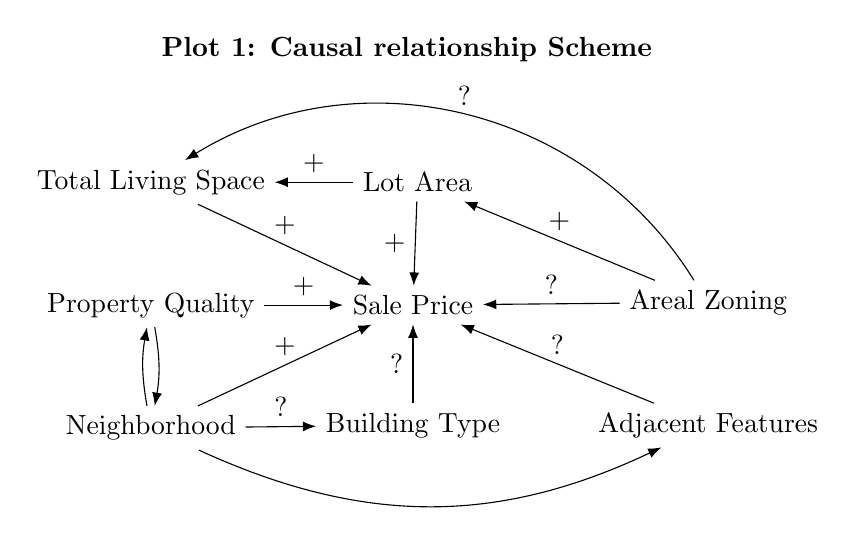
\begin{tikzpicture}
	\centering
 	\node at (3.25,3.25) {\textbf{Plot 1: Causal relationship Scheme}};
    \node (1) at (0,0) {Property Quality};
	\node (2) [above = of 1] {Total Living Space};
	\node (3) [right = of 1] {Sale Price};
	\node (4) [below = of 3] {Building Type};
	\node (5) [right = of 4] {Adjacent Features};
	\node (6) [above = of 5] {Areal Zoning};
	\node (7) [below = of 1] {Neighborhood};
	\node (8) [right = of 2] {Lot Area};
	
	\path (7) edge node[above] {$+$} (3);
	% \path (7) edge node[left] {$?$} (2);
	\path (7) edge[bend left=10](1);
	\path (1) edge[bend left=10](7);
	\path (8) edge node[above] {$+$}(2);
	\path (2) edge node[above] {$+$}(3);
	\path (1) edge node[above] {$+$}(3);
	\path (8) edge node[left] {$+$}(3);
	\path (4) edge node[left] {$?$}(3);
	\path (7) edge node[above] {$?$}(4);
	\path (6) edge node[above] {$+$}(8);
	\path (7) edge[bend right=25](5);
	\path (5) edge node[above] {$?$}(3);
	\path (6) edge node[above] {$?$}(3);
	\path (6) edge[bend right=45] node[above] {$?$}(2);

\end{tikzpicture}
\end{center}


\indent Based on the valuation strategies and EDA discussed above, a theory was set up to explain the variation in sales prices. The corresponding causal relationship scheme can be seen in Plot 1. 

\indent \paragraph{} \textbf{Plot XXX} displays a potential direct positive association between Total Living Space (IV) and Sale Price (DV). Thus, one expects that larger houses have a higher sale price. Consequently,we assume that:

\begin{hyp}[H\ref{hyp:first}] \label{hyp:first}
Total living space (IV) has a direct postive association with Sales Price (DV)
\end{hyp}

\begin{center}
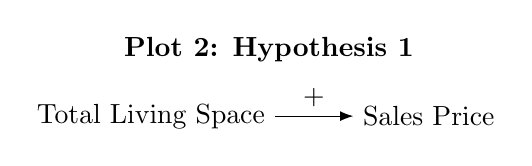
\begin{tikzpicture}
	\centering
 	\node at (1.5,0.85) {\textbf{Plot 2: Hypothesis 1}};
 	\node (1) at (0,0) {Total Living Space};
	\node (2) [right = of 1] {Sales Price};
	\path (1) edge node[above] {$+$}(2);
\end{tikzpicture}
\end{center}


\indent \paragraph{} Subsequently, when taking the Zoning (MSZoning or MSZoning\_grouped - IV) into account to reflect the administrative borderrs of the Ames districts, larger houses in more densly populated areas of the city appear to have a lower price when compared to houses of same size in less densly populated areas as can be seen in \textbf{Plot XXXX2}. This suggests a separation between "downtown less affluent areas" and "suburban affluent areas"\footnote{As an extention\: we will test whether the groups of Neighborhoods generally stay in the same zoning category; if Neighborhoods and Zoning are not related (so eg 50 \% of one neighborhood is in rural zone while the other part is in moderately populated zone) then we have a problem that this woudl induce a bias. Otherwise, we can just proceed.} and concludes in the hypothesis that

\begin{hyp}[H\ref{hyp:second}] \label{hyp:second}
Zoning moderates (MIV) the direct postive association of Total Living Space (IV) and Sale Price (DV). The association of Space and Sale Price is proposed to be weaker for more densly populated areas than for more rural areas. 
\end{hyp}

\begin{center}
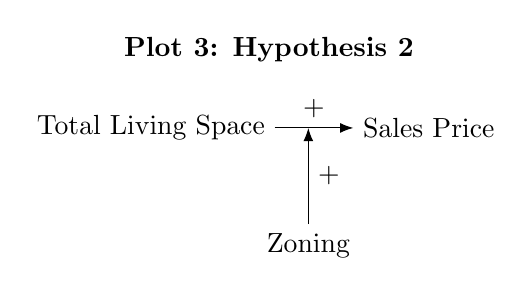
\begin{tikzpicture}
	\centering
 	\node at (1.5,1) {\textbf{Plot 3: Hypothesis 2}};
 	\node (1) at (0,0) {Total Living Space};
	\node (2) [right = of 1] {Sales Price};
	\node (3) at (2,-1.5) {Zoning};
	
	\coordinate (4) at (2,0);
	
	\path (1) edge node[above] {$+$}(2);
	\path (3) edge node[right] {$+$}(4);
\end{tikzpicture}
\end{center}


\indent \paragraph{} As the previous hypothesis suggested, location may be an important factor in explaining the variance in Sale Price. The assumption that affluent houses tend to cluster in afluent neighborhoods is, thus, close. We can thus assume that afluent neighborhood tend to pose the best qualitative propertie. As was discovered during the EDA in part 1, Quality (IV) has a positive association with Sale Price (DV). Subsequently, this research investigates to what extend this clustering differs for the different Neighborhood(s) (IV). \textbf{However, due to Neighborhood not being a suitable variable for this analysis, Zoning again is used as a proxy.}

\begin{hyp}[H\ref{hyp:third}] \label{hyp:third}
Neighborhood of a property moderates the relationship of Quality on Sales Price. Neighborhoods tend to cluster and display simiar patterns observed.\footnote{This hypothesis is partially meant to show the problematic of clustering in the data; this will be further investigated in part 3 \& 4 of this research assignment}


\end{hyp}

\begin{center}
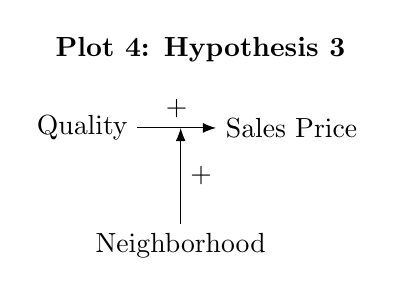
\begin{tikzpicture}
	\centering
 	\node at (1.5,1) {\textbf{Plot 4: Hypothesis 3}};
 	\node (1) at (0,0) {Quality};
	\node (2) [right = of 1] {Sales Price};
	\node (3) at (1.25,-1.5) {Neighborhood};
	
	\coordinate (4) at (1.25,0);
	
	\path (1) edge node[above] {$+$}(2);
	\path (3) edge node[right] {$+$}(4);
\end{tikzpicture}
\end{center}



FURTHERMORE, a possible fourht hypothesis pertains to the capital that has to be invested upon buying the house; such as remodeling etc. This value is assumed to be larger for houses that have not been remodeled for along time before being sold. As such, the foruth hypothesis states that (ADDITIONALLY, we assume this relationship to hold for neighborhoods as well! so neighborhoods doe not ahve an impact here)

\begin{hyp}[H\ref{hyp:fourth}] \label{hyp:fourth}
Years Since Last Remodelling (IV) has a negative association with Sale Price (DV)
\textbf{IMPORTANT! ZONING MAY BE AN ALTERNATIVE TO NEIGHBORHOOD HERE WHICH WOULD MAKE THE ANALYSIS WAY EASIER IN GENERAL}
\end{hyp}

\begin{center}
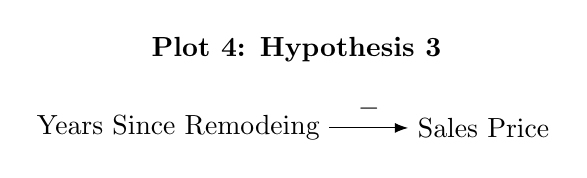
\begin{tikzpicture}
	\centering
 	\node at (1.5,1) {\textbf{Plot 4: Hypothesis 3}};
 	\node (1) at (0,0) {Years Since Remodeing};
	\node (2) [right = of 1] {Sales Price};


	
	\path (1) edge node[above] {$-$}(2);

\end{tikzpicture}
\end{center}




\begin{center}
$ {SalePrice} = \alpha + \beta_{1} TotLivingSpace - \beta_{2}  TotLivingSpace^2 + \beta_{3}  Quality + \beta_{4}  Zoning_{Low Density} + \beta_{5}  Zoning_{Other} + \beta_{6}  YearsSinceRemodeling + \beta_{7}  LotArea + \beta_{8} TotLivingSpace*Zoning_{Low Density} + \beta_{9} TotLivingSpace*Zoning_{Other} +\epsilon$
\end{center}

\textbf{IMPORTANT: DO YOU INCLUDE A QUADRATIC TERM IN THE POPULATION REGRESSION MODEL????}
\begin{center}
$ {SalePrice} = \alpha + \beta_{1} TotLivingSpace - \beta_{2}  TotLivingSpace^2 + \beta_{3}  Quality + \beta_{4}  Zoning - \beta_{5}  YearsSinceRemodeling + \beta_{6}  LotArea + \beta_{7} TotLivingSpace*Zoning + \beta_{8} AdjacentFeatures + \beta_{9} BuildingType \epsilon$
\end{center}




\indent \paragraph{Assumtions for Linear Regression} Considering the population regression model above, the first assumptions requires a linear relationship between the independent and the dependent variables. As could be observed during the EDA in part 1, this assumtion is likely to hold, with a weak nonliear relationship of Total Living Area and Sale Price; this can be rectivfied using a quadratic term. 

https://statisticsbyjim.com/regression/ols-linear-regression-assumptions/

A1: Linearity of model parameters and error term; through the formulation of the (population) regression model, addressing the models' functional form. Thus, a violation of this assumtion is practically impossible if the functional for of the population regression is defined correctly. 

A2: desribes that for a linear system to be solvable, no independent variable can be a linear function of other independent variables. This implies that for dummy varaibles to have one "comparative" category to be droped. furthermore, the "almost" failure of this assumtion, multicollinearity also brings problems with it. While some multicollinearity is to be expected between the coeficients; strong multicollinearity leads to a lower precision in the estimate. Further tests will be conducted to probe for this assumption violation. 

A3: This assumption is referred to as mean independence (or exogeniety); assuming no correlation/systematic association between independent variables and residuals (or conditional mean error is dependent on independent variables). However,as could be seen during the EDA in part 1, the linearity assumption holds for most of the variables we have observed except for a weak quadratic relationship. 
Thus this assumption might induce a bais/ or reduce consistency of the estimator; this is why this assumption must be treated with care. but it is also difficult to be found as omitted variable bias is very likely to have occured during this issue; one example might be crime which has an impact on whether a certain neighborhood is afluent or not.

A4: The error term has a constant variance for each observation expected! --> heteroscedasticity

Generally, as the sample size increases, this assumption becomes less important for the estimate itself, considering that OLS is a consistent estimator; which is the case here (N is quite large). However, heteroscedastictiy may lead to problems regarding inference, as the standard error of the estimate may still be biased. As such, solutions will be later implemented to control for such violations.


A5: Data generation: xi can be random or fixed

A6: Normal distribution of disturbanc (The error term is normally distributed. generally, the means that the error term has a population mean of zeor and standard errror of 1. Generally, most distributions tend to approach normal distributions as sample sizes increase. For some distirbutions such as Sales Price (which is of a financial nature), this can also be remedied through tra´nsforming (here apply log transform). Additionally, multiple controls and test will be conducted down the line to investiate this issue.






\section{OLS regression and model fit}






\end{document}